\chapter{Evaluation}
\label{eval}

\section{Introduction}
In this chapter the two implemented techniques will be evaluated under three read world workloads. In order to show the effect of each configuration parameter, multiple experiments have been designed and deployed. Table~\ref{des:tab:config} defines the configuration space. First, characteristics of workload will be discussed in Section~\ref{eval:workload}. Thereafter, there is separate section for each experiment. Finally, Section~\ref{eval:conc} concludes this chapter.

\section{Workload Characteristic}
\label{eval:workload}

DEBS 2014~\cite{debs2014} has been chosen as a real world workload to test the implementation. Each workload contains data from a random location of the original workload and replayed to feed Spark cluster. All experiments were run for one hour. Figure~\ref{eval:fig:workload} shows distribution of messages in three workloads which have been captured from Spark UI.
\begin{figure}
    \centering
      \begin{subfigure}[h]{\linewidth}
        \centering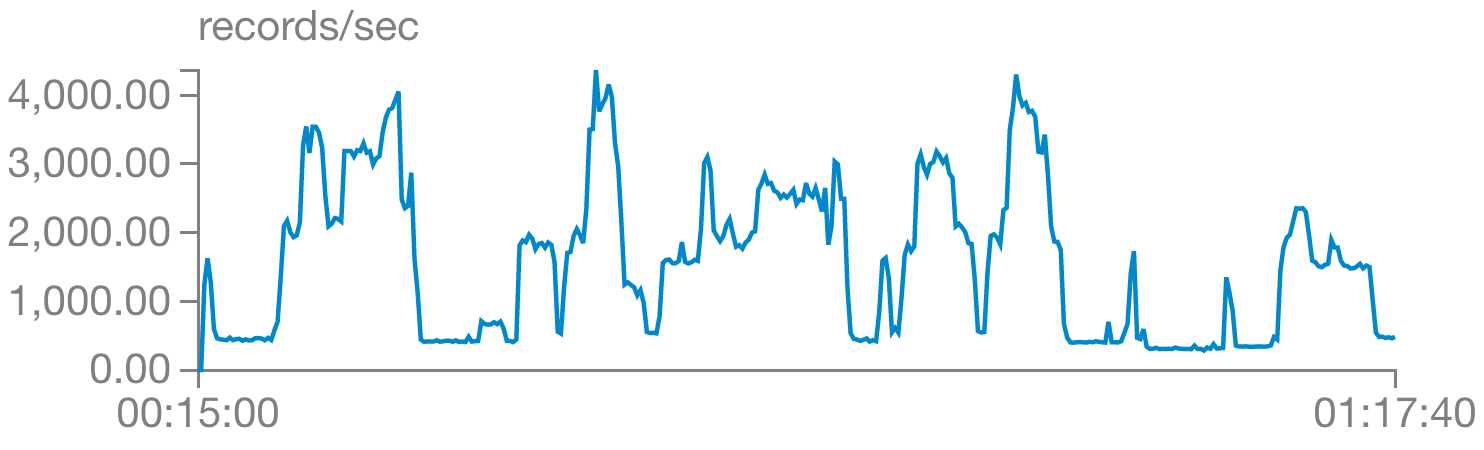
\includegraphics[scale=0.6]{workload1.png}
        \caption{Workload 1}
    \end{subfigure}
    \begin{subfigure}[h]{\linewidth}
        \centering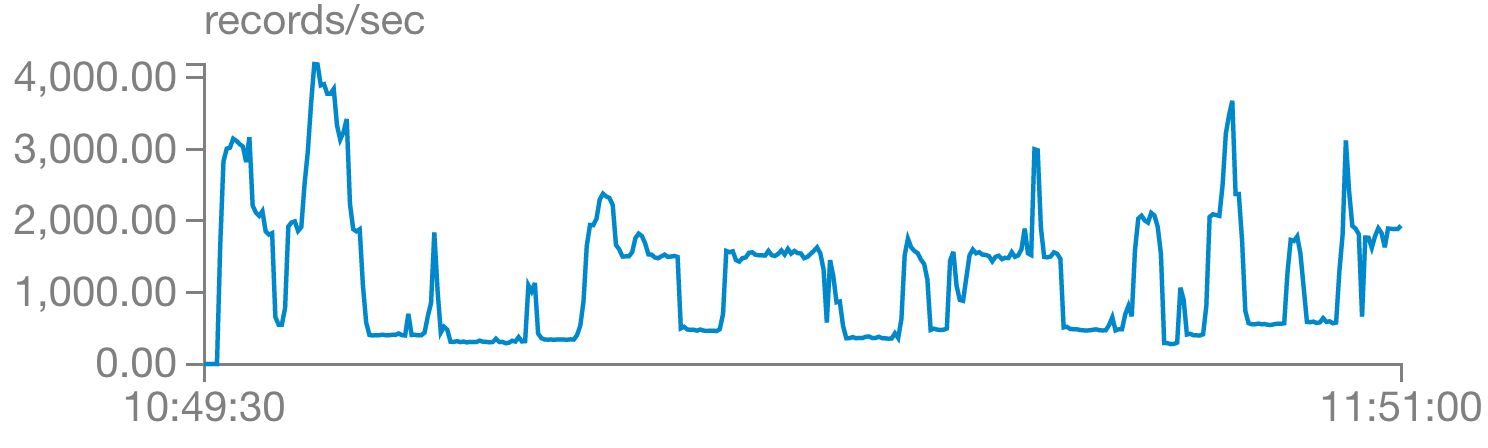
\includegraphics[scale=0.6]{workload2.png}
        \caption{Workload 2}
    \end{subfigure}
    \caption{Three Workloads of DEBS 2014}
    \label{eval:fig:workload}
\end{figure}

The workload involves sensors that measure energy consumption of devices. Each device is connected to one household which in turn is located in one house. This creates a hierarchy from house as parent of households and household as parent of devices. The workload asks to predict energy consumption per device, per household, and per house  for next window of time. The prediction runs over a sliding window of historical measurements which contains $n$ elements. Assuming $window$ variable contains $n$ elements of the history, Equation~\ref{eval:l:pred} defines how the predicted value is calculated.
\begin{equation}
\text{predicted value} = \frac{\text{average(window)} + \text{median(window)}}{2}
\label{eval:l:pred}
\end{equation}

In all experiments \emph{batch size} is set to 10 seconds. The cluster uses 24 executors with minimum of 4 executors that should be respected by Auto-Scaler. All experiments start with minimum number of executors -- 4 in this case -- and run for \emph{one} hour. In case any training is required to run the experiment, training data set is separated from the original workload dataset.

In order to make each workload CPU intensive enough, window size is changed for each workload. Table~\ref{eval:tab:history} defines the history window size for each workload.
\begin{table*}[h]
    \begin{tabular}{lc}
        \toprule
        \textbf{Workload} & \textbf{Window Size = $n$ }\\
        \midrule
        Workload 1 & 1650\\
        Workload 2 & 2050\\
        Workload 3 & 2050\\
        \bottomrule
    \end{tabular}
    \centering
    \caption{Workload Window Size}
    \label{eval:tab:history}
\end{table*}

\clearpage
\section{Experiment 3: Executor Strategy}
This experiment has been designed to illustrate the strategy of adding/removing executors when taking Scale-In or Scale-Out actions. Table~\ref{eval:tab:ex3} shows the configuration this experiment.
\begin{table}[h]
    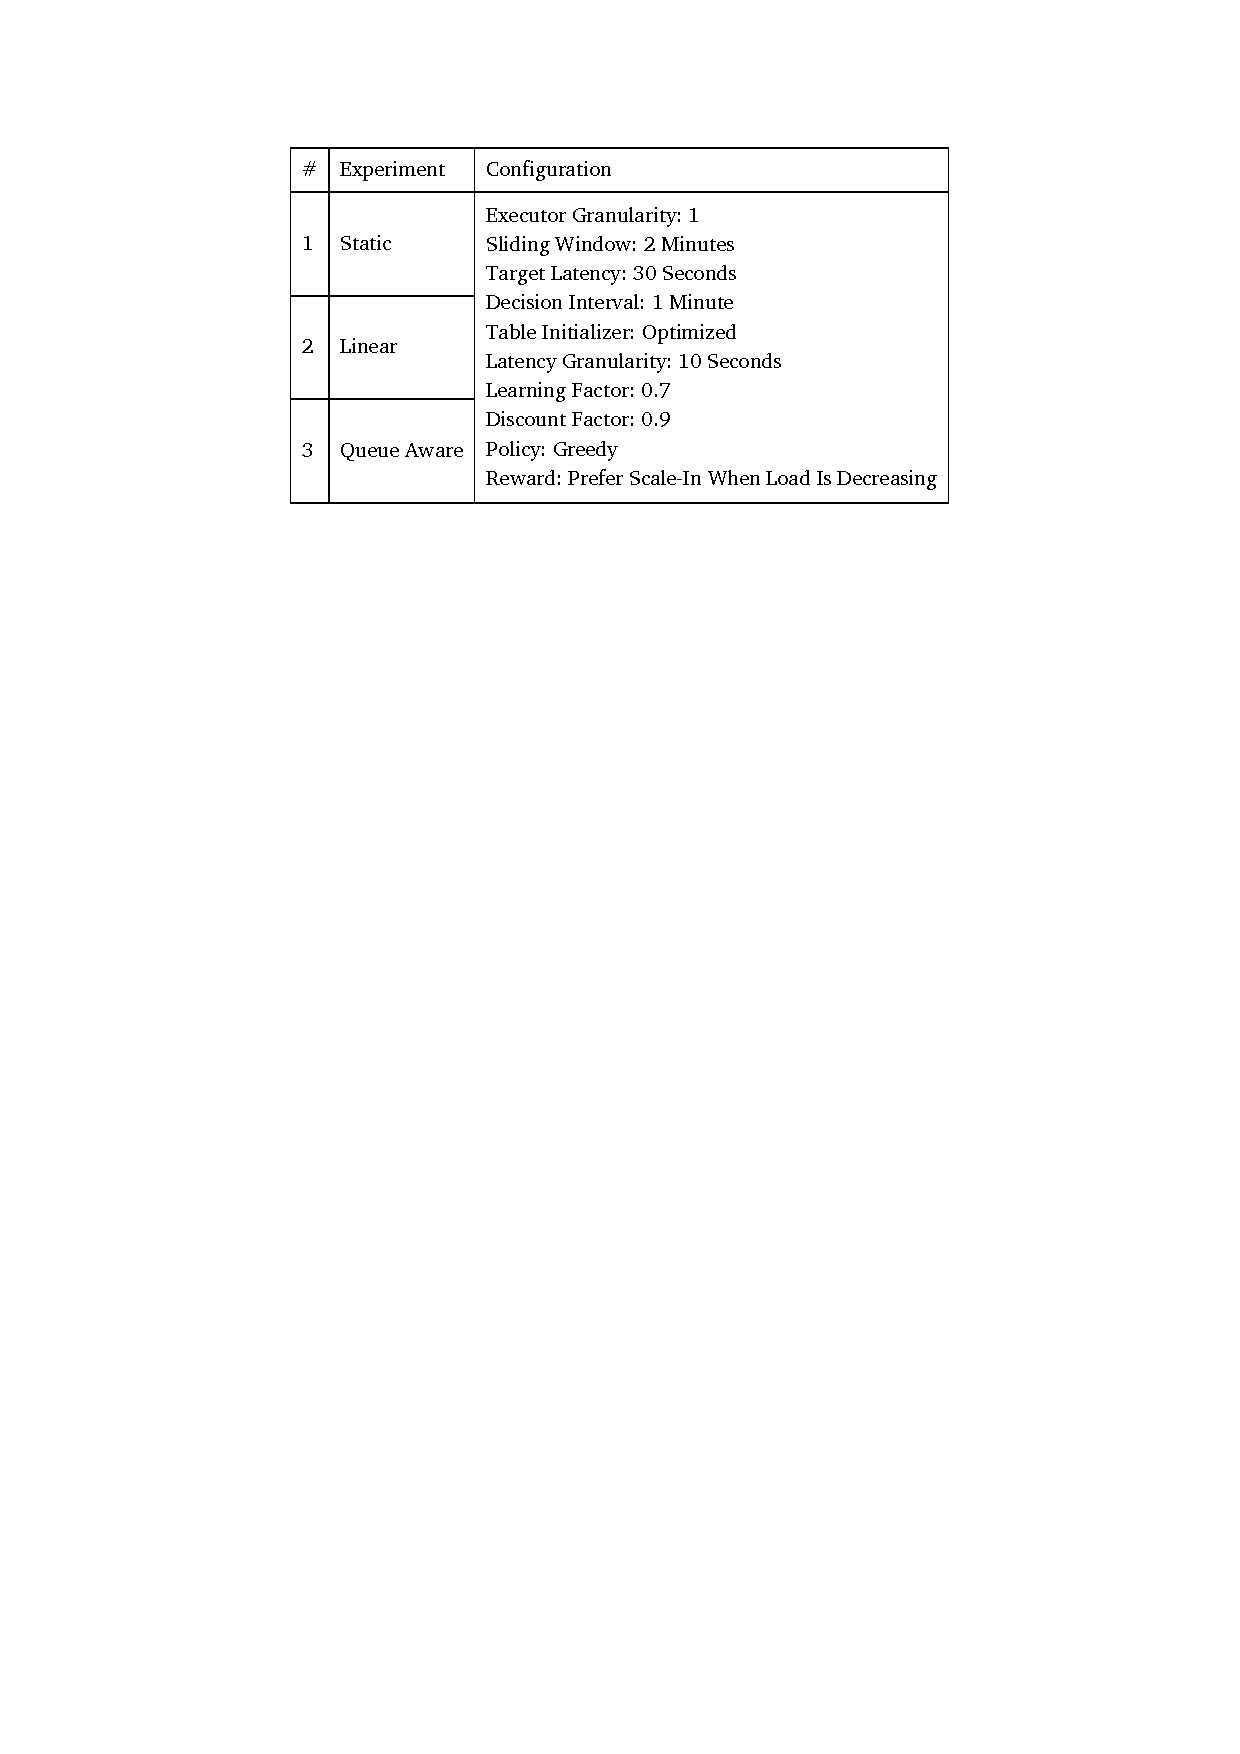
\includegraphics[clip,trim=4.7cm 21.18cm 4.7cm 2.5cm]{tables/ex3.pdf}
    \centering
    \caption{Executor Strategy Configuration Parameters}
    \label{eval:tab:ex3}
\end{table}

\subsection{Workload 1}

\subsection{Workload 2}

\subsection{Workload 3}

\section{Conclusion}
\label{eval:conc}